%%%%%%%%%%%%%%%%%%%%%%%%%%%%%%%%%%%%%%%%%%%%%%%%%%%%%%%%%%%%%%%%%%%%%%%%%%%

\documentclass{standalone}

\usepackage{amsmath}
\usepackage{mathptmx}
\usepackage{pgfplots}
\usetikzlibrary{external}
\tikzexternalize{e-1200-growth-rate}
\pgfplotsset{compat=1.15}

%% IEEE uses Times Roman font, so we'll default to Times.
%% These three commands make up the entire times.sty package.
\renewcommand{\rmdefault}{ptm}
\renewcommand{\ttdefault}{pcr}
\normalfont\selectfont

\begin{document}

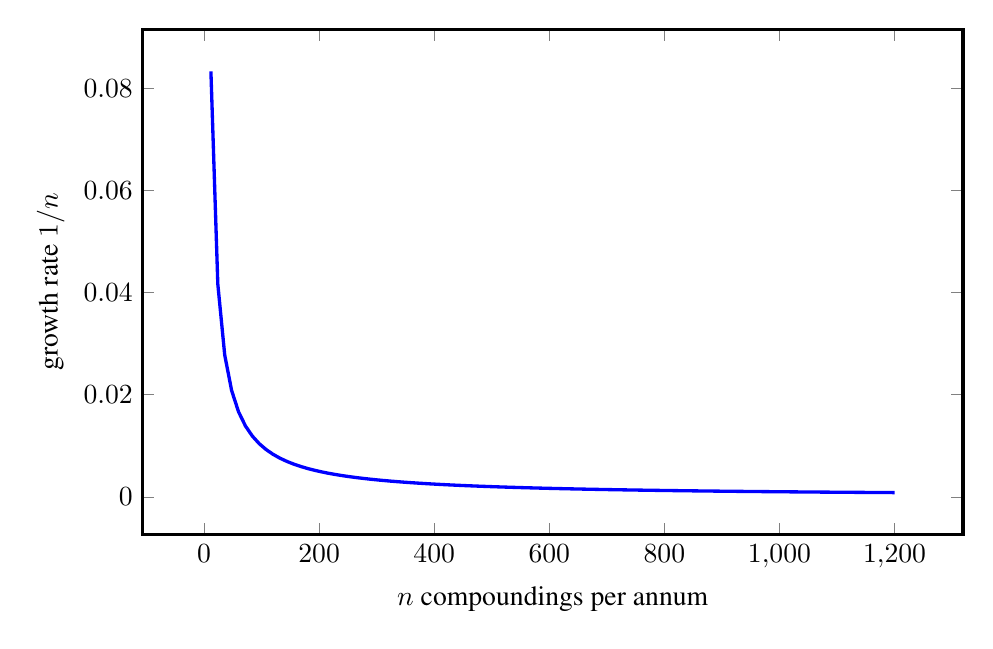
\begin{tikzpicture}
\tikzset{%%
  every mark/.append style={scale=1.0},%%
  scale=1.0%%
}
\pgfplotsset{%%
  every axis/.append style={font=\normalsize}%%
}
%%
\begin{axis}[%%
  axis line style=very thick,%%
  dotStyle/.style={very thick,blue,mark=none},%%
  enlargelimits=true,%%
  height=8cm,%%
  plotStyle/.style={%%
    domain=4:17,%%
    mark=none,%%
    smooth,%%
    thick%%
  },%%
  width=12cm,%%
  %% x axis
  xlabel={\normalsize $n$ compoundings per annum},%%
  %% y axis
  ylabel={\normalsize growth rate $1 / n$},%%
  scaled y ticks=false,%%
  y tick label style=/pgf/number format/fixed%%
]
%%
%%
\addplot[dotStyle] coordinates {
  (12, 0.083333333333333)
  (24, 0.041666666666667)
  (36, 0.027777777777778)
  (48, 0.020833333333333)
  (60, 0.016666666666667)
  (72, 0.013888888888889)
  (84, 0.011904761904762)
  (96, 0.010416666666667)
  (108, 0.009259259259259)
  (120, 0.008333333333333)
  (132, 0.007575757575758)
  (144, 0.006944444444444)
  (156, 0.006410256410256)
  (168, 0.005952380952381)
  (180, 0.005555555555556)
  (192, 0.005208333333333)
  (204, 0.004901960784314)
  (216, 0.00462962962963)
  (228, 0.004385964912281)
  (240, 0.004166666666667)
  (252, 0.003968253968254)
  (264, 0.003787878787879)
  (276, 0.003623188405797)
  (288, 0.003472222222222)
  (300, 0.003333333333333)
  (312, 0.003205128205128)
  (324, 0.003086419753086)
  (336, 0.00297619047619)
  (348, 0.002873563218391)
  (360, 0.002777777777778)
  (372, 0.002688172043011)
  (384, 0.002604166666667)
  (396, 0.002525252525253)
  (408, 0.002450980392157)
  (420, 0.002380952380952)
  (432, 0.002314814814815)
  (444, 0.002252252252252)
  (456, 0.00219298245614)
  (468, 0.002136752136752)
  (480, 0.002083333333333)
  (492, 0.002032520325203)
  (504, 0.001984126984127)
  (516, 0.001937984496124)
  (528, 0.001893939393939)
  (540, 0.001851851851852)
  (552, 0.001811594202899)
  (564, 0.00177304964539)
  (576, 0.001736111111111)
  (588, 0.001700680272109)
  (600, 0.001666666666667)
  (612, 0.001633986928105)
  (624, 0.001602564102564)
  (636, 0.001572327044025)
  (648, 0.001543209876543)
  (660, 0.001515151515152)
  (672, 0.001488095238095)
  (684, 0.001461988304094)
  (696, 0.001436781609195)
  (708, 0.001412429378531)
  (720, 0.001388888888889)
  (732, 0.001366120218579)
  (744, 0.001344086021505)
  (756, 0.001322751322751)
  (768, 0.001302083333333)
  (780, 0.001282051282051)
  (792, 0.001262626262626)
  (804, 0.001243781094527)
  (816, 0.001225490196078)
  (828, 0.001207729468599)
  (840, 0.001190476190476)
  (852, 0.001173708920188)
  (864, 0.001157407407407)
  (876, 0.001141552511416)
  (888, 0.001126126126126)
  (900, 0.001111111111111)
  (912, 0.00109649122807)
  (924, 0.001082251082251)
  (936, 0.001068376068376)
  (948, 0.001054852320675)
  (960, 0.001041666666667)
  (972, 0.001028806584362)
  (984, 0.001016260162602)
  (996, 0.001004016064257)
  (1008, 0.000992063492063)
  (1020, 0.000980392156863)
  (1032, 0.000968992248062)
  (1044, 0.00095785440613)
  (1056, 0.00094696969697)
  (1068, 0.000936329588015)
  (1080, 0.000925925925926)
  (1092, 0.000915750915751)
  (1104, 0.000905797101449)
  (1116, 0.00089605734767)
  (1128, 0.000886524822695)
  (1140, 0.000877192982456)
  (1152, 0.000868055555556)
  (1164, 0.00085910652921)
  (1176, 0.000850340136054)
  (1188, 0.000841750841751)
  (1200, 0.000833333333333)
};
\end{axis}
\end{tikzpicture}

\end{document}
